\documentclass[10pt,conference]{IEEEtran}
% If the IEEEtran.cls has not been installed into the LaTeX system files,
% manually specify the path to it:
% \documentclass[conference]{../sty/IEEEtran}
\usepackage{graphicx}
\usepackage{subcaption}
\begin{document}

% paper title
\title{Identification of black hole states using matrix based methods: Time series analysis of RXTE satellite data}


% author names and affiliations
% use a multiple column layout for up to three different
% affiliations
%\author{
%\authorblockN{A. Chockalingam}
%\authorblockA{Dept.\ of Electrical Communication Engg.\\
%Indian Institute of Science \\
%Bangalore, 560012, India\\
%Email: spcom2016@gmail.com} \and
%\authorblockN{Rahul Vaze}
%\authorblockA{School of Technology and Computer Science\\
%Tata Institute of Fundamental Research\\
%Mumbai, 400005, India\\
%Email: spcom2016@gmail.com}
%\and
%\authorblockN{Animesh Kumar}
%\authorblockA{Dept.\ of Electrical Engg.\\
%Indian Institute of Technolgy \\
%Bombay, 400076, Mumbai India\\
%Email: spcom2016@gmail.com} 
%%\and
%%\authorblockN{Robert Calderbank}
%%\authorblockA{Department of Electrical Engineering\\
%%Princeton University \\
%%Princeton, NJ 08544, USA\\
%%Email: calderbk@math.princeton.edu} \and
%%\authorblockN{Habong Chung}
%%\authorblockA{Department of Electronic\\
%%\& Electrical Engineering\\
%%Hongik University\\
%%Seoul, Korea\\
%%Email: habchung@hongik.ac.kr}
%}
% avoiding spaces at the end of the author lines is not a problem with
% conference papers because we don't use \thanks or \IEEEmembership
% for over three affiliations, or if they all won't fit within the width
% of the page, use this alternative format:
% make the title area
\maketitle

\begin{abstract}
Black hole is one of the fascinating,  however mysterious, astro-physical  objects. In order to identify it one has to look at its environment, often forming a disc-like structure. This disc, called accretion disc, evolves with time transiting from one state to another. For example, in one extreme regime it shows temperature dependent radiations making the disc geometrically thin, and in other extreme  regime of time span however radiation turns out to be temperature independent making the disc hot and geometrically thick.  Nevertheless in general accretion disc lies in a state intermediate between the two extremes. The present mission is to capture black hole states  explicitly using PCA and SVD based decompositions. In order to do that we rely on time series data of black hole GRS 1915 +105 obtained from RXTE satellite. As a black hole cannot be seen directly, identifying its states accurately could help in characterizing its properties. Earlier time series  analysis based on correlation dimension methods, supplemented by theory, argued for four specific states. However there are caveats when data themselves are not free from noise and the  appropriate method for such an analysis itself is exploratory. Present interdisciplinary study aims at, on one hand to cross-verify the previous inference, on the other hand to identify, if any,  novel characteristics of black holes. This is expected to have long standing implications in astrophysics and otherwise.
\end{abstract}

\section{Introduction}


\section{Related Work}


\section{Proposed Method}
In this work, we use two different matrix based approaches to characterize time series as stochastic vs non-stochastic.

\begin{itemize}
  \item PCA Based approach: In the first approach, we utilize PCA to understand if the available data occupy a preferred orientation. This can be computed by splitting the time series into two halves, and computing the covariance matrix of these observations. The eigen values of this $2 \times 2$ covariance matrix will show one of the signatures : If the data indeed shows any preferred direction (as in Non-stochastic time series), then the larger eigen value will be significantly greater than the other. This will lead to a large ratio of the eigen values. On the other hand, if the data does not show any preferred direction (as in Stochastic time series), then the two eigen values of the covariance matrix will be comparable. This will lead to small values of eigen value ratio.


  Consider a segment of time series consisting of $n$ values  $z_1, z_2 \mathellipsis z_n$.  Covariance matrix, $C$, for this interval is computed as the covariance between two vectors $(z_1, z_2 \mathellipsis z_{\frac{n}{2}})$ and $(z_\frac{n}{2}, \mathellipsis z_n)$. Finally eigen values, $\lambda_1$ and $\lambda_2$ of $C$, which satisfies equation \ref{eqn:eig_ratio}, are computed and the eigen ratio is computed as  $\frac{\lambda_1}{\lambda_2}$ where $\lambda_1 \ > \lambda_2$.
  \begin{equation}
   Cv_i = \lambda_{i}v_i
    \label{eqn:eig_ratio}
  \end{equation}
  \item SVD based approach: In this approach, we form uncorrelated observation vectors from the raw time series data by utilizing optimal value of embedding dimension \cite{misra2006}. A data matrix, $D$, is formed with each row  as the  time shifted version of the original time series signal. The time shift is chosen to be large enough so that each row can be viewed as a different observation vector of the same phenomenon. The temporal dynamics is understood by utilizing the right singular vectors of the SVD decomposition of the data matrix as given in equation \ref{eqn:svd}. Columns of $U$ and $V$  form the left and right singular vectors and $\Sigma$ is a diagonal matrix with diagonal elements as the singular values.
\begin{equation}
  D = U \Sigma V^T
  \label{eqn:svd}
\end{equation}
   The plot of pair-wise observation vectors is compared against the plot of the top two right singular vectors.
\end{itemize}

Using PCA analysis we derived the following three features:
\begin{itemize}
  \item Maximum eigen ratio: This is the maximum value obtained as the ratio of the two eigen values of the covariance matrix of any sub-interval of the time series.
  \item Variance of eigen ratio: This is the variance of the eigen ratios of covariance matrices across sub-interval in the entire time series.
  \item Area under the eigen ratio curve: This measure captures the area under the curve of the eigen ratio for the entire time series.
\end{itemize}

\section{Results and Discussions}

\begin{figure*}[ht]
%\begin{subfigure}{1\textwidth}
  \centering
  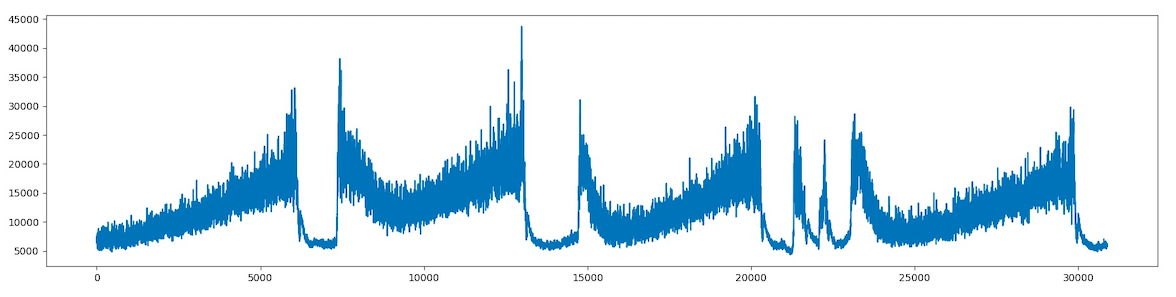
\includegraphics[width=\linewidth]{theta_ts.png}
  \caption{A representative of stochastic time series signal}
  \label{theta_ts}
\end{figure*}
\begin{figure*}[ht]
%\begin{subfigure}{1\textwidth}
  \centering
  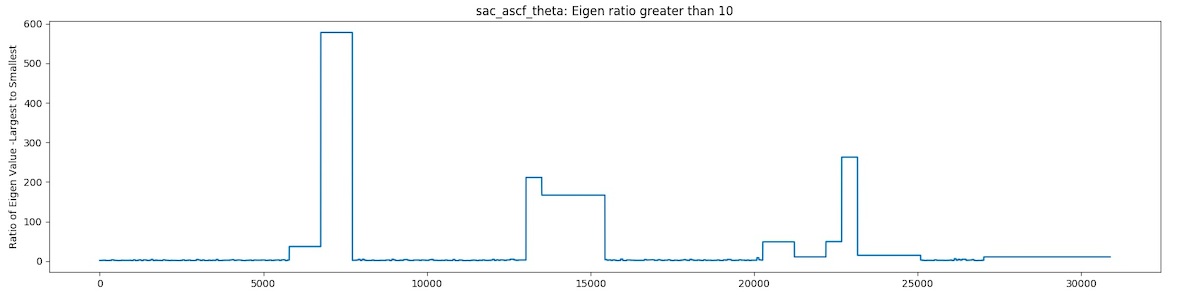
\includegraphics[width=\linewidth]{theta_ts_eig.png}
  \caption{Plot of eigen ratio of the  stochastic time series shown in Figure \ref{theta_ts}}
  \label{theta_eig}
\end{figure*}


In our experiments we noticed the following behavior for each of the above features:
\begin{itemize}
  \item Eigen ratio values are small across the entire time series, typically lying in the range 1 - 20. This implies the maximum eigen ratio value will also be small. On the other hand, for the non-stochastic time series the eigen ratio values are significantly high, typically reaching a few thousands in certain sub-intervals. Hence the maximum eigen ratio value for a non-stochastic time series is typically large.
  \item Variance of eigen ratios: For a stochastic signal since the range of eigen ratio values is typically small, the variance is also small. On the other hand, for a non-stochastic signal, since the eigen ratio values occupy a large range of values, their variance is typically high.
  \item Area under the eigen ratio curve: For a stochastic time series, since the eigen ratio values are small the area under the curve is also small. However, for a non-stochastic signal the eigen ratio values remain high for longer time intervals. Hence the area under the curve is significantly higher.
\end{itemize}

The above characteristics have been exploited in the present study to distinguish between stochastic vs non-stochastic signal.

\begin{table*}[t]
\caption{Time series: comparison between correlation dimension behavior vs proposed PCA features }
\begin{center}
\begin{tabular}{|c|c|c|c|c|c|c|c|c|}
\hline
Class & CD-Behavior & Diskbb & PL & MER & Variance & Area & Inference & Match\\
\hline
$\beta$ & F & 46 & 52 & 214 & 483 & 43 & Non-stochastic & Yes \\
\hline
$\theta$ & F &  & & 577 & 778 & 58&Non-stochastic & Yes \\
\hline
$\lambda$ & F & 54 & 46 & 600 & 6782 & 314 & Non-stochastic & Yes \\
\hline
$\kappa$ & F & 59 & 51 & 700 & 5199 & 144 & Non-stochastic & Yes \\
\hline
$\mu$ & F & 56 & 41 & 50 & 51 & 12 & Non-stochastic & Yes \\
\hline
$\nu$ & F & 28 & 72 & 30 & 32 & 16 & Non-stochastic & Yes \\
\hline
$\alpha$ & F & 23 & 77 & 30 & 1.9 & 27.7 & Non-stochastic & Yes \\
\hline
$\rho$ & LC & 28 & 72 & 60 & 147 & 35 & Non-stochastic & Yes \\
\hline
$\delta$ & S & 48 & 50 & 42 & 9.74 & 26.2 & Non-stochastic & No \\
\hline
$\phi$ & S & 50 & 34 & 7 & 0.5 & 15 & Stochastic & Yes \\
\hline
$\gamma$ & S & 60 & 31 & 12 & 1 & 16 & stochastic & Yes \\
\hline
$\chi$ & S & 09 & 89 & 5.6 & 0.25 & 6.05 & Stochastic & Yes \\
\hline
\end{tabular}
\label{tab:results}
\end{center}
\end{table*}

From table \ref{tab:results} we notice that for time series of most classes the inference using PCA based features matches with  that observed using correlation dimension based approach. However, for certain classes of time series such as $\delta$ time series there is a conflict between the inferences using the two methods (TODO).

\subsection{SVD based approach}

\begin{figure}[ht]
%\begin{subfigure}{1\textwidth}
  \centering
  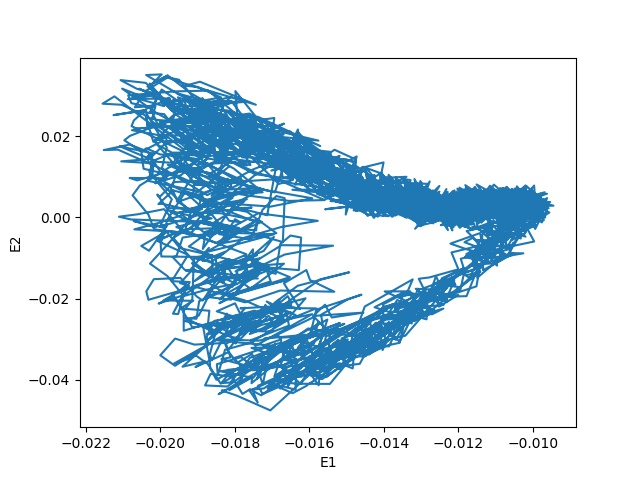
\includegraphics[width=\linewidth]{rho_svd.jpg}
  \caption{Plot of E1 Vs E2 (top two right singular vectors) of data matrix for  time seres $\rho$}
  \label{svd}
\end{figure}

From SVD decomposition of the data matrix, we pick up the top 2 right singular vectors (E1, E2) corresponding to the temporal dynamics.
From the figure we notice that the behavior observed in the E1 vs E2 plot is consistent with the characteristic of the time series (TODO).


\begin{figure*}[ht]
%\begin{subfigure}{1\textwidth}
  \centering
  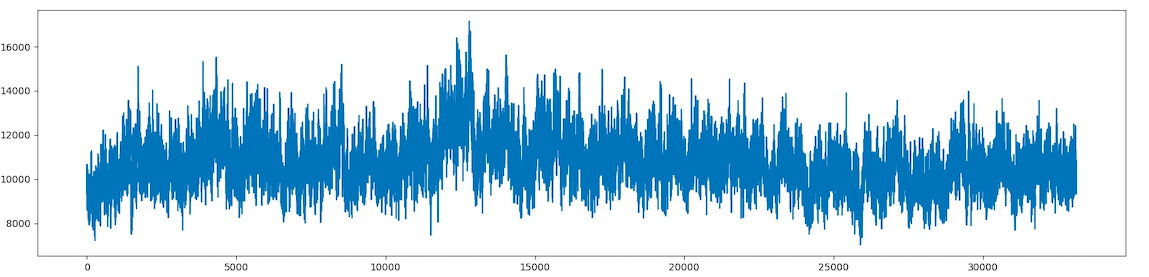
\includegraphics[width=0.9\linewidth]{phi_ts.png}
  \caption{A representative of non-stochastic time series signal}
  \label{phi_ts}
%\end{subfigure}
  \end{figure*}

\begin{figure*}[ht]

%\begin{subfigure}{1\textwidth}
  \centering
  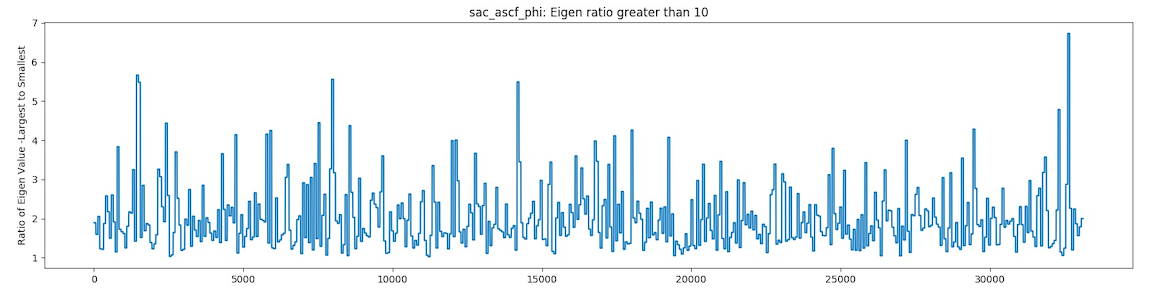
\includegraphics[width=0.9\linewidth]{phi_ts_eig.png}
  \caption{Plot of eigen ratio of the non-stochastic signal shown in Figure \ref{phi_ts}}
  \label{phi_eig}
%\end{subfigure}
\end{figure*}

\begin{figure}
    \centering
    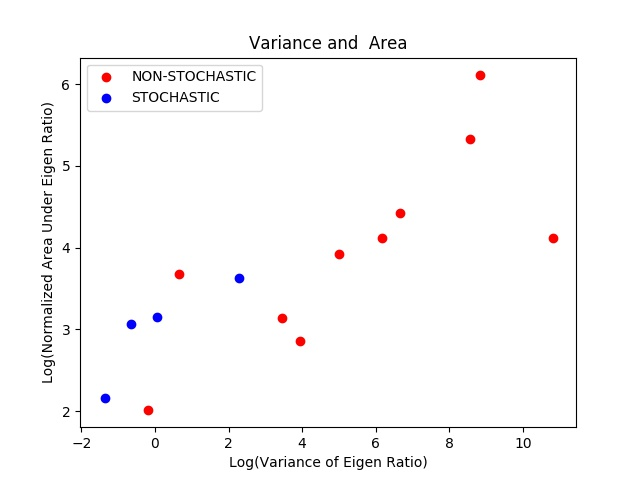
\includegraphics[width=.9\linewidth]{variance_area.jpg}
    \caption{Feature space (variance and area) shows that the two classes are well separated}
    \label{figure11}
\end{figure}

\section{Conclusion}
Conclusions, if any, go here.

% conference papers do not normally have an appendix


\begin{thebibliography}{1}

\bibitem{misra2006}
Misra, Ranjeev, et al. "The nonlinear behavior of the black hole system grs 1915+ 105." The Astrophysical Journal 643.2 (2006): 1114.

\bibitem{Boaretto2021}
Boaretto, B. R. R., et al. "Discriminating chaotic and stochastic time series using permutation entropy and artificial neural networks." Scientific reports 11.1 (2021): 1-10.

\bibitem{lacasa2010}
  Lacasa, Lucas, and Raul Toral. "Description of stochastic and chaotic series using visibility graphs." Physical Review E 82.3 (2010): 036120.
\bibitem{Adegoke2018}
Adegoke, Oluwashina, et al. "Correlating non-linear properties with spectral states of RXTE data: possible observational evidences for four different accretion modes around compact objects." Monthly Notices of the Royal Astronomical Society 476.2 (2018): 1581-1595.

\end{thebibliography}


\end{document}
